%% 
%% Copyright 2007-2025 Elsevier Ltd
%% 
%% This file is part of the 'Elsarticle Bundle'.
%% ---------------------------------------------
%% 
%% It may be distributed under the conditions of the LaTeX Project Public
%% License, either version 1.3 of this license or (at your option) any
%% later version.  The latest version of this license is in
%%    http://www.latex-project.org/lppl.txt
%% and version 1.3 or later is part of all distributions of LaTeX
%% version 1999/12/01 or later.
%% 
%% The list of all files belonging to the 'Elsarticle Bundle' is
%% given in the file `manifest.txt'.
%% 
%% Template article for Elsevier's document class `elsarticle'
%% with numbered style bibliographic references
%% SP 2008/03/01
%% $Id: elsarticle-template-num.tex 272 2025-01-09 17:36:26Z rishi $
%%
\documentclass[preprint,12pt]{elsarticle}

%% Use the option review to obtain double line spacing
%% \documentclass[authoryear,preprint,review,12pt]{elsarticle}

%% Use the options 1p,twocolumn; 3p; 3p,twocolumn; 5p; or 5p,twocolumn
%% for a journal layout:
%% \documentclass[final,1p,times]{elsarticle}
%% \documentclass[final,1p,times,twocolumn]{elsarticle}
%% \documentclass[final,3p,times]{elsarticle}
%% \documentclass[final,3p,times,twocolumn]{elsarticle}
%% \documentclass[final,5p,times]{elsarticle}
%% \documentclass[final,5p,times,twocolumn]{elsarticle}

%% For including figures, graphicx.sty has been loaded in
%% elsarticle.cls. If you prefer to use the old commands
%% please give \usepackage{epsfig}

%% The amssymb package provides various useful mathematical symbols
\usepackage{amssymb}
%% The amsmath package provides various useful equation environments.
\usepackage{amsmath}
%% The amsthm package provides extended theorem environments
%% \usepackage{amsthm}

%% The lineno packages adds line numbers. Start line numbering with
%% \begin{linenumbers}, end it with \end{linenumbers}. Or switch it on
%% for the whole article with \linenumbers.
%% \usepackage{lineno}

\journal{Nuclear Physics B}

\begin{document}

\begin{frontmatter}

%% Title, authors and addresses

%% use the tnoteref command within \title for footnotes;
%% use the tnotetext command for theassociated footnote;
%% use the fnref command within \author or \affiliation for footnotes;
%% use the fntext command for theassociated footnote;
%% use the corref command within \author for corresponding author footnotes;
%% use the cortext command for theassociated footnote;
%% use the ead command for the email address,
%% and the form \ead[url] for the home page:
%% \title{Title\tnoteref{label1}}
%% \tnotetext[label1]{}
%% \author{Name\corref{cor1}\fnref{label2}}
%% \ead{email address}
%% \ead[url]{home page}
%% \fntext[label2]{}
%% \cortext[cor1]{}
%% \affiliation{organization={},
%%             addressline={},
%%             city={},
%%             postcode={},
%%             state={},
%%             country={}}
%% \fntext[label3]{}

\title{}

%% use optional labels to link authors explicitly to addresses:
%% \author[label1,label2]{}
%% \affiliation[label1]{organization={},
%%             addressline={},
%%             city={},
%%             postcode={},
%%             state={},
%%             country={}}
%%
%% \affiliation[label2]{organization={},
%%             addressline={},
%%             city={},
%%             postcode={},
%%             state={},
%%             country={}}

\author{} %% Author name

%% Author affiliation
\affiliation{organization={},%Department and Organization
            addressline={}, 
            city={},
            postcode={}, 
            state={},
            country={}}

%% Abstract
\begin{abstract}
%% Text of abstract
World models have demonstrated strong capability in learning dynamical systems from high-dimensional observations, but often lack interpretability and physical grounding. The Physically Interpretable World Model (PIWM) addresses this limitation by learning latent representations that correspond to meaningful physical state variables while preserving accurate prediction of system dynamics.

The proposed framework integrates a visual encoder, a structured latent representation, and a dynamics model trained under weak supervision to enforce physically consistent behavior. Through this design, PIWM is able to recover interpretable latent states and achieve accurate prediction performance across multiple control environments.

In this journal version, we extend the original work by providing a more comprehensive evaluation of the model’s predictive behavior and interpretability. In particular, we analyze performance across different trajectory segments, investigate the impact of data inconsistencies on prediction error, and study the model’s behavior under varying conditions. Additionally, we provide deeper insight into the role of relative representations and latent dynamics in improving generalization.

These extensions offer a more complete understanding of the strengths and limitations of PIWM, highlighting its potential for physically grounded modeling in autonomous systems.

 
\end{abstract}


%%Graphical abstract
\begin{graphicalabstract}
%\includegraphics{grabs}
\end{graphicalabstract}

%%Research highlights
\begin{highlights}
\item Research highlight 1
\item Research highlight 2
\end{highlights}

%% Keywords
\begin{keyword}
%% keywords here, in the form: keyword \sep keyword

%% PACS codes here, in the form: \PACS code \sep code

%% MSC codes here, in the form: \MSC code \sep code
%% or \MSC[2008] code \sep code (2000 is the default)

\end{keyword}

\end{frontmatter}

%% Add \usepackage{lineno} before \begin{document} and uncomment 
%% following line to enable line numbers
%% \linenumbers

%% main text
%%

%% Use \section commands to start a section

%%introduction

\section{Introduction}
    World models have emerged as a powerful paradigm for learning the dynamics of complex systems directly from high-dimensional observations such as images. By encoding visual inputs into compact latent representations and modeling their temporal evolution, these approaches enable prediction, planning, and control across a wide range of applications, including robotics and autonomous driving. Despite their strong predictive performance, however, most existing world models operate as black-box systems, where the learned latent representations lack clear physical meaning. As a result, it is difficult to interpret, diagnose, or trust the model’s predictions, particularly in safety-critical settings.

A central challenge in world modeling is to learn representations that are both predictive and physically meaningful. Conventional approaches typically optimize latent spaces for reconstruction accuracy or forecasting performance, without enforcing any explicit correspondence between latent variables and underlying physical quantities such as position, velocity, or orientation. Consequently, even when predictions appear visually accurate, they may not reflect physically consistent system behavior. This limitation reduces the reliability of learned models and hinders their ability to generalize across different environments or operating conditions.

The Physically Interpretable World Model (PIWM) framework addresses this limitation by introducing structured latent representations that are explicitly aligned with meaningful physical variables while preserving accurate prediction of system dynamics. By combining visual encoding with a physics-aware latent structure and training under weak supervision, PIWM enables the recovery of interpretable latent states without requiring access to exact ground-truth physical annotations. This provides a promising direction for improving both the transparency and robustness of learned world models.

In this work, we extend the PIWM framework through a detailed empirical study in a realistic autonomous driving setting using the Donkey Car simulator. While prior work has demonstrated the feasibility of learning physically interpretable representations, a deeper understanding of how these representations behave under practical conditions remains limited. In particular, questions regarding generalization, sensitivity to data quality, and the role of trajectory structure in prediction performance have not been thoroughly explored.

To address these gaps, we introduce a trajectory-based learning and evaluation framework that leverages sliding-window sequence modeling and relative coordinate representations. By expressing vehicle motion in a local reference frame, the proposed approach reduces dependence on global position and orientation, enabling improved generalization across different regions of the track. In addition, we systematically analyze prediction performance across trajectory segments and investigate the impact of data inconsistencies on model accuracy.

Our study provides new insights into the behavior of physically grounded world models in real-world-like conditions. In particular, we show that prediction errors are strongly influenced by irregularities in the underlying data, and that when evaluated on consistent trajectory segments, the model achieves highly accurate motion prediction. These findings highlight the importance of both representation design and data quality in achieving reliable and interpretable world modeling.

 






\section{Method for Donkey Car}
\label{sec1}
\subsection{Dataset and Window Construction}

The dataset consists of driving trajectories collected from the Donkey Car simulator.  Each timestep contains an RGB camera frame, the control actions applied to the vehicle, and the corresponding ground truth vehicle state. The state vector is defined as

\begin{equation}
s_t = (x_t, y_t, \psi_t, v_t)
\end{equation}

where $x_t$ and $y_t$ represent the global vehicle position, $\psi_t$ denotes the yaw angle (in degrees), and $v_t$ is the vehicle speed.

To train the model, the trajectory is converted into fixed-length sliding windows. Each window contains 15 consecutive timesteps and is generated with a stride of 5 frames.  Thus, the starting index of each window is

\begin{equation}
t_0 \in \{0, 5, 10, 15, \ldots\}
\end{equation}

and the window spans

\begin{equation}
[t_0, t_0 + 14]
\end{equation}

This approach produces overlapping samples that preserve temporal continuity while 
increasing the number of training examples.

\subsection{Context--Target Prediction Setup}

Each window is divided into a context sequence and a prediction target.

The first 14 frames form the input context:

\begin{equation}
(x_{t_0}, x_{t_1}, \ldots, x_{t_{13}})
\end{equation}

along with the corresponding control actions. The final frame of the window serves as the prediction target:

\begin{equation}
x_{t_{14}}
\end{equation}

Thus, the model performs a 14-step input to 1-step output prediction task, where the network must infer the future vehicle motion based on the preceding observations and actions.

\subsection{Relative Coordinate Representation}

Instead of predicting absolute global coordinates, the model predicts the vehicle displacement relative to the first frame of the window. For a window beginning at time $t_0$, the global displacement is defined as

\begin{equation}
\Delta x = x_{t_{14}} - x_{t_0}
\end{equation}

\begin{equation}
\Delta y = y_{t_{14}} - y_{t_0}
\end{equation}

To remove dependence on global orientation, this displacement is rotated into the local coordinate frame of the vehicle at time $t_0$. Using the initial yaw angle $\psi_{t_0}$, the relative coordinates are computed as

\begin{equation}
x_r = \cos(\psi_{t_0})\Delta x + \sin(\psi_{t_0})\Delta y
\end{equation}

\begin{equation}
y_r = -\sin(\psi_{t_0})\Delta x + \cos(\psi_{t_0})\Delta y
\end{equation}

This representation allows the model to learn motion dynamics independent of global position or orientation, improving generalization across the track.

\subsection{Model Architecture}

The model consists of three jointly trained components: a variational autoencoder (VAE), a latent predictor, and a state extraction network.

\paragraph{Variational Autoencoder}

Each input frame is encoded into a latent representation using a variational autoencoder:

\begin{equation}
z_t = Encoder(x_t)
\end{equation}

The latent dimension used in the experiments is $z_t \in \mathbb{R}^{64}$. During training and evaluation, the mean of the latent distribution ($\mu$) is used as the deterministic representation of the image.

\paragraph{Latent Sequence Predictor}

The sequence of latent vectors from the context frames is passed to an LSTM-based predictor together with the control actions:

\begin{equation}
(z_{t_0}, z_{t_1}, \ldots, z_{t_{13}})
\end{equation}

The predictor models the temporal dynamics of the vehicle and produces a prediction of the next latent state:

\begin{equation}
\hat{z}_{t_{14}}
\end{equation}

\paragraph{State Extraction Network}

A small feedforward network maps the predicted latent representation to the relative 
vehicle displacement:

\begin{equation}
(\hat{x}_r, \hat{y}_r) = f(\hat{z}_{t_{14}})
\end{equation}

This produces the final predicted motion of the vehicle in the local coordinate frame.

\subsection{Training Objective}

The model is trained jointly using three loss components. The first is the VAE reconstruction loss, which ensures that the latent representation preserves visual information. The second is the latent prediction loss, which encourages the LSTM predictor to accurately forecast the next latent state. The third is the relative position loss, which measures the error between predicted and ground truth 
relative displacements:

\begin{equation}
L_{xy} = \left\| (\hat{x}_r, \hat{y}_r) - (x_r, y_r) \right\|^2
\end{equation}

\subsection{Evaluation Metric}

Model performance is evaluated using the root mean squared error (RMSE) of the 
predicted relative displacement. For $N$ prediction windows, the RMSE is defined as

\begin{equation}
RMSE = \sqrt{\frac{1}{N} \sum_{i=1}^{N} \left((\hat{x}_{r,i} - x_{r,i})^2 + (\hat{y}_{r,i} - y_{r,i})^2\right)}
\end{equation}

\subsection{Experimental Results}

Using the described architecture and training procedure, the model achieved the 
following prediction accuracy on the dataset:

\begin{itemize}
\item RMSE$_x$ = 0.057 m
\item RMSE$_y$ = 0.048 m
\item RMSE$_{xy}$ = 0.075 m
\end{itemize}

This corresponds to an average positional prediction error of approximately 
7.5 cm for a one-step prediction based on a 14-frame observation context. 

\subsection{Best-Lap Analysis}

During evaluation, prediction error was computed across all laps of the recorded trajectory. While most laps exhibited consistent prediction performance, several laps contained abnormally large errors due to inconsistencies in the recorded trajectory data.  Inspection of these laps revealed occasional irregularities in the state measurements,  which likely arose from noise or logging artifacts in the dataset.

To better evaluate the predictive capability of the model under normal operating conditions, a best-lap analysis was performed. The lap with the lowest prediction error was identified and analyzed separately. For this lap, the model achieved a relative displacement error of

\[
RMSE_{xy} = 0.0238 \; \text{m}
\]

which corresponds to approximately 2.4 cm of positional error.

Figure~\ref{fig:best_lap} shows the predicted trajectory compared to the ground truth vehicle path.

\begin{figure}[h]
\centering
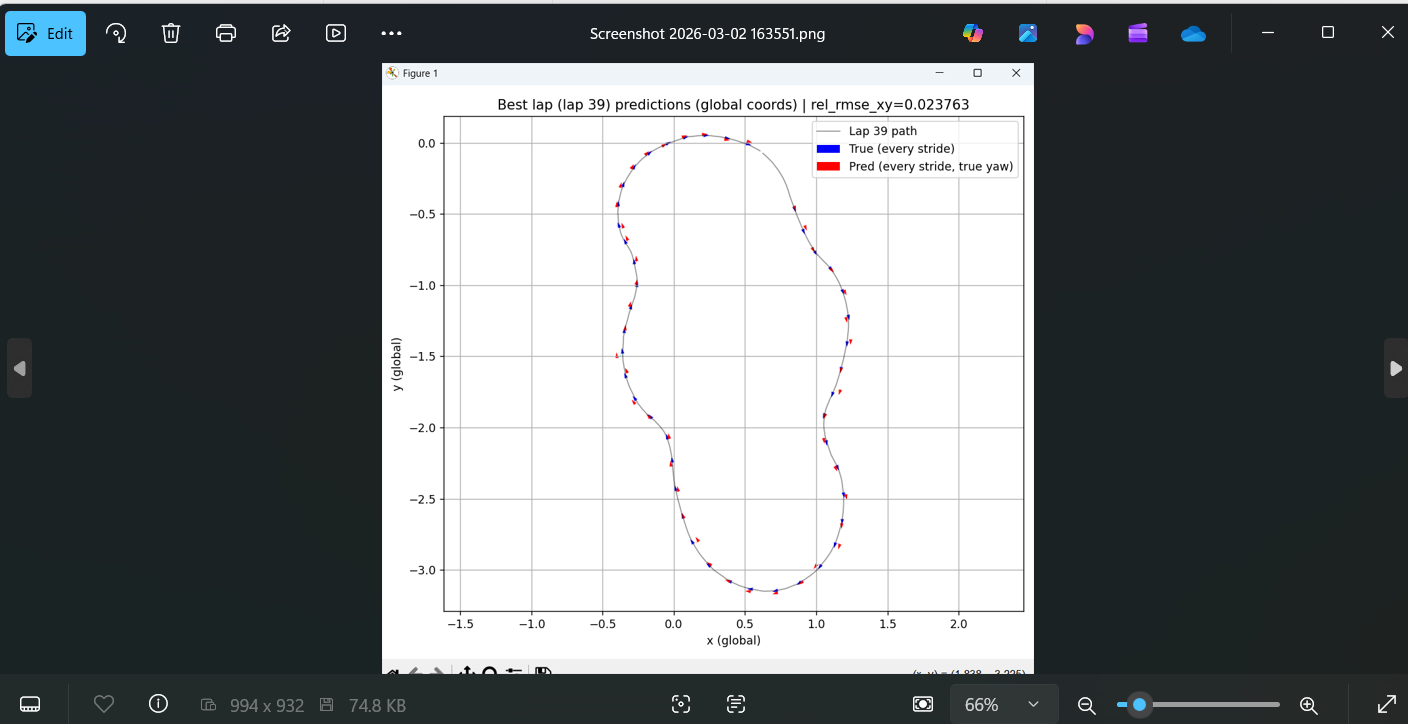
\includegraphics[width=0.8\linewidth]{donkeycarbestlap.png}
\caption{Predicted trajectory compared with the ground truth path for the best-performing lap.}
\label{fig:best_lap}
\end{figure}compared to the ground  truth vehicle path for this lap. The predicted displacements closely follow the true trajectory, demonstrating that the model is capable of accurately capturing the vehicle's motion dynamics when trained on consistent trajectory segments.

The higher errors observed in other laps are therefore attributed primarily to data irregularities rather than limitations of the model itself. When evaluated on clean trajectory segments, the model maintains low prediction error and accurately reconstructs the vehicle path.

\subsection{Multi-Step Prediction and Long-Horizon Evaluation }

To further evaluate the predictive capability of the model beyond single-step forecasting, we extend the framework to perform \textbf{multi-step trajectory prediction} over longer horizons.

Instead of predicting only the next timestep, the model is recursively applied to generate future states over multiple steps. At each timestep, the predicted latent representation is fed back into the model along with the corresponding control inputs to produce the next prediction. This autoregressive process allows the model to simulate the evolution of the vehicle trajectory over an extended horizon.

Formally, given an initial context window:
\begin{equation}
(z_{t_0}, z_{t_1}, \dots, z_{t_{13}})
\end{equation}
the model predicts:
\begin{equation}
\hat{z}_{t_{14}}, \hat{z}_{t_{15}}, \dots, \hat{z}_{t_{14+H}}
\end{equation}
where $H$ is the prediction horizon. The predicted latent states are mapped to relative displacements using the state extraction network and accumulated to reconstruct the predicted trajectory in global coordinates.

\subsection{Evaluation of Long-Horizon Predictions}

Long-horizon performance is evaluated by comparing the predicted trajectory to the ground truth trajectory over complete laps. The root mean squared error (RMSE) is computed across all predicted points:
\begin{equation}
RMSE = \sqrt{ \frac{1}{N} \sum_{i=1}^{N} \left( (\hat{x}_i - x_i)^2 + (\hat{y}_i - y_i)^2 \right) }
\end{equation}

Figure~\ref{fig:long_horizon} shows representative examples of predicted trajectories for several laps. The predicted trajectories closely follow the ground truth path, demonstrating that the model is able to maintain accurate motion estimates over extended time horizons.

Across different laps, the model achieves long-horizon RMSE values in the range of approximately $0.05$--$0.07$ meters, indicating that prediction errors remain bounded even as the prediction horizon increases.

\subsection{Observations on Long-Horizon Behavior}

Analysis of the predicted trajectories reveals several important characteristics:

\begin{itemize}
    \item \textbf{Stable trajectory tracking:} The model maintains close alignment with the ground truth path over most segments of the track.

    \item \textbf{Error accumulation in high-curvature regions:} Slight deviations are observed in sharp turns, where small prediction errors accumulate over time.

    \item \textbf{Robustness across laps:} Despite variations in trajectory segments, the model consistently produces physically plausible motion patterns.
\end{itemize}

These results demonstrate that the learned latent dynamics capture not only short-term motion but also \textbf{long-term trajectory structure}, which is critical for downstream tasks such as planning and control.

\section{Analysis}

In this section, we provide a detailed analysis of the model's predictive behavior, focusing on trajectory-level performance, the impact of data quality, and the role of the proposed representation in improving generalization.

\subsection{Effect of Relative Coordinate Representation}

A key component of the proposed approach is the use of relative coordinate representations, where future motion is expressed in the local coordinate frame of the vehicle. By removing dependence on global position and orientation, this formulation allows the model to focus on learning underlying motion dynamics rather than memorizing absolute spatial locations.

Empirically, this representation leads to improved generalization across different regions of the track. Because similar motion patterns (e.g., turns and straight segments) are expressed consistently in the local frame, the model is able to reuse learned dynamics across trajectories. This reduces sensitivity to variations in global pose and enables more stable predictions over long horizons.

\subsection{Trajectory-Level Prediction Behavior}

To better understand model performance beyond aggregate metrics, we analyze predictions at the level of complete trajectories. Figure~\ref{fig:long_horizon} illustrates representative long-horizon predictions across multiple laps.

The results show that the model is able to closely track the ground truth trajectory over extended time horizons. In most segments of the track, the predicted trajectory remains well aligned with the true path, indicating that the learned latent dynamics capture the overall structure of vehicle motion.

However, small deviations can be observed, particularly in regions of high curvature. These deviations arise from the accumulation of small prediction errors over time, which become more pronounced during sharp turns where accurate modeling of vehicle dynamics is more challenging.

\subsection{Impact of Data Inconsistencies}

An important observation from our experiments is the significant impact of data quality on prediction performance. While most trajectory segments yield consistent and accurate predictions, certain laps exhibit noticeably higher error.

Further inspection reveals that these high-error cases correspond to irregularities in the recorded state data, likely caused by sensor noise or logging artifacts. These inconsistencies introduce discrepancies between the visual observations and the associated state labels, making it more difficult for the model to learn a consistent mapping.

To isolate the model's performance under ideal conditions, we perform a best-lap analysis, selecting the trajectory segment with the lowest prediction error. For this segment, the model achieves a substantially lower RMSE compared to the dataset average, demonstrating that the underlying model is capable of highly accurate motion prediction when trained on consistent data.

This finding highlights that prediction error is not solely determined by model capacity, but is strongly influenced by the quality and consistency of the training data.

\subsection{Long-Horizon Stability and Error Accumulation}

The long-horizon evaluation reveals that prediction errors remain relatively small and bounded over time, despite the autoregressive nature of the prediction process. This indicates that the learned latent dynamics are stable and do not exhibit significant drift.

Nevertheless, error accumulation is still present, particularly in challenging segments such as sharp turns. These errors are primarily due to compounding inaccuracies in the predicted latent states, which propagate through subsequent predictions.

Despite this, the model consistently produces physically plausible trajectories, suggesting that the learned representation captures meaningful structure in the underlying dynamics.

\subsection{Discussion of Latent Dynamics}

The combination of a learned latent representation and a sequence predictor enables the model to capture both visual and dynamical aspects of the system. The latent space encodes information relevant to vehicle motion, while the temporal model learns how this representation evolves over time.

The results indicate that this formulation is sufficient to model short-term and long-term motion patterns without explicit supervision on physical variables. This supports the central idea of PIWM, where structured latent representations can capture physically meaningful behavior even under weak supervision.

Overall, the analysis demonstrates that the proposed approach achieves a balance between predictive accuracy and physical consistency, while also revealing the importance of representation design and data quality in determining model performance. 


\section{Example Section}
\label{sec1}
%% Labels are used to cross-reference an item using \ref command.

Section text. See Subsection \ref{subsec1}.

%% Use \subsection commands to start a subsection.
\subsection{Example Subsection}
\label{subsec1}

Subsection text.

%% Use \subsubsection, \paragraph, \subparagraph commands to 
%% start 3rd, 4th and 5th level sections.
%% Refer following link for more details.
%% https://en.wikibooks.org/wiki/LaTeX/Document_Structure#Sectioning_commands

\subsubsection{Mathematics}
%% Inline mathematics is tagged between $ symbols.
This is an example for the symbol $\alpha$ tagged as inline mathematics.

%% Displayed equations can be tagged using various environments. 
%% Single line equations can be tagged using the equation environment.
\begin{equation}
f(x) = (x+a)(x+b)
\end{equation}

%% Unnumbered equations are tagged using starred versions of the environment.
%% amsmath package needs to be loaded for the starred version of equation environment.
\begin{equation*}
f(x) = (x+a)(x+b)
\end{equation*}

%% align or eqnarray environments can be used for multi line equations.
%% & is used to mark alignment points in equations.
%% \\ is used to end a row in a multiline equation.
\begin{align}
 f(x) &= (x+a)(x+b) \\
      &= x^2 + (a+b)x + ab
\end{align}

\begin{eqnarray}
 f(x) &=& (x+a)(x+b) \nonumber\\ %% If equation numbering is not needed for a row use \nonumber.
      &=& x^2 + (a+b)x + ab
\end{eqnarray}

%% Unnumbered versions of align and eqnarray
\begin{align*}
 f(x) &= (x+a)(x+b) \\
      &= x^2 + (a+b)x + ab
\end{align*}

\begin{eqnarray*}
 f(x)&=& (x+a)(x+b) \\
     &=& x^2 + (a+b)x + ab
\end{eqnarray*}

%% Refer following link for more details.
%% https://en.wikibooks.org/wiki/LaTeX/Mathematics
%% https://en.wikibooks.org/wiki/LaTeX/Advanced_Mathematics

%% Use a table environment to create tables.
%% Refer following link for more details.
%% https://en.wikibooks.org/wiki/LaTeX/Tables
\begin{table}[t]%% placement specifier
%% Use tabular environment to tag the tabular data.
%% https://en.wikibooks.org/wiki/LaTeX/Tables#The_tabular_environment
\centering%% For centre alignment of tabular.
\begin{tabular}{l c r}%% Table column specifiers
%% Tabular cells are separated by &
  1 & 2 & 3 \\ %% A tabular row ends with \\
  4 & 5 & 6 \\
  7 & 8 & 9 \\
\end{tabular}
%% Use \caption command for table caption and label.
\caption{Table Caption}\label{fig1}
\end{table}


%% Use figure environment to create figures
%% Refer following link for more details.
%% https://en.wikibooks.org/wiki/LaTeX/Floats,_Figures_and_Captions
\begin{figure}[t]%% placement specifier
%% Use \includegraphics command to insert graphic files. Place graphics files in 
%% working directory.
\centering%% For centre alignment of image.
\includegraphics{example-image-a}
%% Use \caption command for figure caption and label.
\caption{Figure Caption}\label{fig1}
%% https://en.wikibooks.org/wiki/LaTeX/Importing_Graphics#Importing_external_graphics
\end{figure}


%% The Appendices part is started with the command \appendix;
%% appendix sections are then done as normal sections
\appendix
\section{Example Appendix Section}
\label{app1}

Appendix text.

%% For citations use: 
%%       \cite{<label>} ==> [1]

%%
Example citation, See \cite{lamport94}.

Robotics and Autonomous Systems (RAS)


Autonomous Robots
%% If you have bib database file and want bibtex to generate the
%% bibitems, please use
%%
%%  \bibliographystyle{elsarticle-num} 
%%  \bibliography{<your bibdatabase>}

%% else use the following coding to input the bibitems directly in the
%% TeX file.

%% Refer following link for more details about bibliography and citations.
%% https://en.wikibooks.org/wiki/LaTeX/Bibliography_Management

\begin{thebibliography}{00}

%% For numbered reference style
%% \bibitem{label}
%% Text of bibliographic item

\bibitem{lamport94}
  Leslie Lamport,
  \textit{\LaTeX: a document preparation system},
  Addison Wesley, Massachusetts,
  2nd edition,
  1994.

\end{thebibliography}
\end{document}

\endinput
%%
%% End of file `elsarticle-template-num.tex'.
